\begin{exercise}
      {ID-323614fb4692457d389583e224a07995486984ea}
      {Dreieck}
  \ifproblem\problem\par
    Gegeben ist ein Quadrat mit der Seitenlänge $a$. Bestimme einen Term $A(x)$,
    mit dem man die Fläche des Dreiecks $ABC$ berechnen kann.
    \begin{center}
      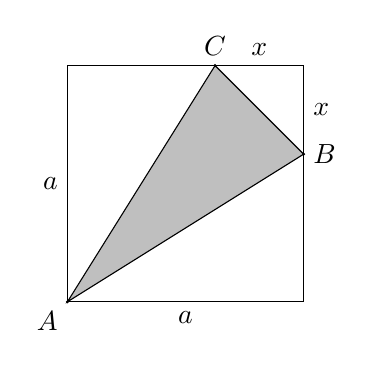
\begin{tikzpicture}[scale=0.75]
        % Dreieck
        \filldraw[fill=black!25!white] (0, 0) -- (4, 2.5) -- (2.5, 4) -- cycle;
        % Eckpunkte
        \fill (0.0, 0.0) circle[radius=0.8pt] node[below left] {$A$};
        \fill (4.0, 2.5) circle[radius=0.8pt] node[right]      {$B$};
        \fill (2.5, 4.0) circle[radius=0.8pt] node[above]      {$C$};
        % Quadrat
        \draw (0, 0) rectangle (4, 4);
        % Seitenlaengen
        \node[left]  at (0.00, 2.00) {$a$};
        \node[below] at (2.00, 0.00) {$a$};
        \node[right] at (4.00, 3.25) {$x$};
        \node[above] at (3.25, 4.00) {$x$};
      \end{tikzpicture}
    \end{center}
  \fi
  %\ifoutline\outline\par
  %\fi
  %\ifoutcome\outcome\par
  %\fi
\end{exercise}
